\chapter{Grundlagen}
\label{ch:grundlagen}

Dieses Kapitel erklärt, was Behavior Cloning vom klassischen Greifen unterscheidet, welche
Schwierigkeiten das Verfahren mit sich bringt und wie die in Modul~4 eingesetzten Verfahren
mathematisch funktionieren. Die Bildverarbeitung und die Robotergrundlagen des klassischen
Ansatzes sind in der Gesamtarbeit beschrieben und werden hier nur so weit aufgegriffen, wie
der Vergleich es erfordert.

% ==============================================================================
\section{Klassischer Ansatz und Behavior Cloning im Vergleich}
\label{sec:vergleich}

\subsection{Klassischer Ansatz}

Beim klassischen Greifen ist die Aufgabe in getrennte, von Hand entworfene Stufen zerlegt
(\cref{fig:vergleich}, oben). Eine Bildverarbeitung bestimmt die Lage des Bauteils, eine
Kalibrierung rechnet sie in Roboterkoordinaten um, und ein Bahnplaner verbindet Start,
Vorgreif-, Greif- und Ablagepose mit programmierten Bewegungen. In der Gesamtarbeit setzen
Modul~1 und Modul~2 genau diese Kette um.

Die Stärken dieses Vorgehens sind Nachvollziehbarkeit und Genauigkeit: Jede Stufe lässt sich
einzeln prüfen, und solange die Annahmen der Bildverarbeitung erfüllt sind, ist das Ergebnis
deterministisch. Die Grenzen liegen in denselben Annahmen. Jede Abweichung, die beim Entwurf
nicht vorgesehen war, etwa eine andere Beleuchtung, ein teilweise verdecktes Bauteil oder eine
verschobene Kamera, muss als eigene Regel ergänzt werden. Außerdem wird die Bahn einmal geplant
und dann ohne Rückkopplung abgefahren (offene Kette): Verrutscht das Bauteil nach der Messung,
greift der Roboter daneben.

\subsection{Behavior Cloning}

Beim Behavior Cloning übernimmt ein neuronales Netz die Abbildung vom Kamerabild auf die
Bewegung als Ganzes (\cref{fig:vergleich}, unten). Statt Regeln zu programmieren, zeigt man
dem System Beispiele der gewünschten Bewegung, und das Netz lernt daraus, in jeder Situation
die passende nächste Aktion auszugeben. Daraus ergeben sich drei Vorteile gegenüber dem
klassischen Ansatz:

\begin{description}
  \item[Keine explizite Zwischendarstellung] Die Lage des Bauteils muss nicht als Zahl
    gemessen werden. Was für das Greifen wichtig ist, lernt das Netz aus den Bildern selbst.
    Kalibrierfehler zwischen Kamera und Roboter wirken sich dadurch weniger aus.
  \item[Geschlossene Regelschleife] Die Policy bewertet in jedem Takt neu, wo das Bauteil
    relativ zum Greifer steht. Abweichungen während der Fahrt kann sie ausgleichen.
  \item[Übertragbarkeit] Für eine neue Aufgabe oder ein neues Bauteil werden neue
    Demonstrationen aufgenommen, die Software bleibt dieselbe.
\end{description}

Der Preis dafür sind der Bedarf an Daten, die schwerere Nachvollziehbarkeit eines gelernten
Verhaltens und eine Reihe grundsätzlicher Schwierigkeiten, die \cref{sec:huerden} beschreibt.

\begin{figure}[htbp]
  \centering
  \begin{tikzpicture}[font=\small, node distance=4mm and 5mm,
      blk/.style={draw, rounded corners=1.5mm, fill=white, align=center, minimum height=11mm,
                  text width=22mm},
      lrn/.style={blk, fill=blue!8, text width=58mm},
      io/.style={blk, fill=black!6, text width=16mm},
      arr/.style={-{Stealth[length=2mm]}, thick}]
    % klassisch
    \node[io] (b1) {Bild};
    \node[blk, right=of b1] (det) {Objekt\-erkennung};
    \node[blk, right=of det] (pose) {Pose in Roboter\-koordinaten};
    \node[blk, right=of pose] (plan) {Bahn\-planung};
    \node[io, right=of plan] (r1) {Roboter};
    \draw[arr] (b1) -- (det); \draw[arr] (det) -- (pose); \draw[arr] (pose) -- (plan);
    \draw[arr] (plan) -- (r1);
    \node[anchor=south west, font=\small\bfseries] at ([yshift=2mm]b1.north west)
      {Klassischer Ansatz (offene Kette)};
    % BC
    \node[io, below=20mm of b1] (b2) {Bild\\+ Zustand};
    \node[lrn, right=of b2] (pol) {gelernte Policy $\pi_\theta$\\(Erkennung und Bewegung in
      einem Netz)};
    \node[io] at (r1 |- pol) (r2) {Roboter};
    \draw[arr] (b2) -- (pol); \draw[arr] (pol) -- node[above, font=\scriptsize] {Aktion $a_t$} (r2);
    \draw[arr, densely dashed] (r2.south) -- ++(0,-6mm) -| node[pos=0.25, below,
      font=\scriptsize] {neue Beobachtung $o_{t+1}$ in jedem Takt} (b2.south);
    \node[anchor=south west, font=\small\bfseries] at ([yshift=2mm]b2.north west)
      {Behavior Cloning (geschlossene Kette)};
  \end{tikzpicture}
  \caption[Klassischer Ansatz und Behavior Cloning]{Klassischer Ansatz mit getrennten,
  programmierten Stufen (oben) und Behavior Cloning mit einer gelernten Abbildung von der
  Beobachtung auf die Aktion, die in jedem Takt neu ausgewertet wird (unten).}
  \label{fig:vergleich}
\end{figure}

% ==============================================================================
\section{Policies und Lernen aus Demonstrationen}
\label{sec:bc-mathe}

\subsection{Begriffe}

Die Steuerung wird als Folge diskreter Takte $t = 0, 1, \dots, T$ betrachtet. In jedem Takt
liegt eine \emph{Beobachtung} $o_t$ vor, in Modul~4 bestehend aus den Kamerabildern und dem
Roboterzustand. Die Policy wählt daraus eine \emph{Aktion} $a_t$, hier die Sollstellung der
Gelenke und den Greiferbefehl für den nächsten Takt. Die Policy ist eine parametrierte
Abbildung
\begin{equation}
  \pi_\theta : o_t \mapsto a_t
  \qquad\text{bzw. stochastisch}\qquad
  a_t \sim \pi_\theta(a \mid o_t),
  \label{eq:policy}
\end{equation}
deren Parameter $\theta$ die Gewichte eines neuronalen Netzes sind. Der Experte, dessen
Verhalten nachgeahmt werden soll, wird mit $\pi^{*}$ bezeichnet. In Modul~4 ist das kein
Mensch, sondern ein Bahnplaner (\cref{ch:datenaufnahme}).

\subsection{Behavior Cloning als überwachtes Lernen}

Aus $N$ Demonstrationen des Experten entsteht ein Datensatz von Paaren
\begin{equation}
  \mathcal{D} = \bigl\{ (o_t^{(i)},\, a_t^{(i)}) \bigr\}_{i = 1 \dots N,\; t = 0 \dots T_i},
  \qquad a_t^{(i)} = \pi^{*}\bigl(o_t^{(i)}\bigr).
\end{equation}
Behavior Cloning behandelt diese Paare wie bei einer gewöhnlichen Regression als voneinander
unabhängige Stichproben und bestimmt die Parameter, die den mittleren Fehler zwischen
vorhergesagter und vorgeführter Aktion minimieren~\cite{pomerleau1989,argall2009,osa2018}:
\begin{equation}
  \theta^{*} = \argmin_{\theta}\;
  \E_{(o, a) \sim \mathcal{D}} \Bigl[ \ell\bigl(\pi_\theta(o),\, a\bigr) \Bigr],
  \qquad \text{z.\,B.}\quad \ell(\hat a, a) = \lVert \hat a - a \rVert_2^2 .
  \label{eq:bc-ziel}
\end{equation}
Eine Belohnungsfunktion wie beim bestärkenden Lernen ist nicht nötig, und das Training
erfolgt vollständig offline auf aufgezeichneten Daten, ohne dass der Roboter dabei fährt.

% ==============================================================================
\section{Hürden des Behavior Cloning}
\label{sec:huerden}

\subsection{Verteilungsverschiebung und Fehlerfortpflanzung}
\label{sec:covariate-shift}

\Cref{eq:bc-ziel} minimiert den Fehler auf den Beobachtungen, die der \emph{Experte}
erzeugt hat, also unter der Verteilung $d_{\pi^{*}}$. Ausgeführt wird aber die gelernte
Policy, und sie erzeugt durch ihre eigenen Aktionen eine andere Verteilung $d_{\pi_\theta}$.
Schon ein kleiner Fehler führt den Roboter in einen Zustand, der in den Demonstrationen nicht
vorkommt; dort ist die Vorhersage unzuverlässiger, der nächste Fehler wird größer, und die
Abweichung schaukelt sich auf (\cref{fig:drift}). Diese Verteilungsverschiebung heißt
\emph{Covariate Shift}.

Ross, Gordon und Bagnell~\cite{ross2011} haben den Effekt quantifiziert. Macht die Policy
auf der Verteilung des Experten in jedem Takt mit Wahrscheinlichkeit $\varepsilon$ einen
Fehler, so sind die Kosten $J$ einer Aufgabe mit $T$ Takten im ungünstigsten Fall
\begin{equation}
  J(\pi_\theta) \;\le\; J(\pi^{*}) + T^{2}\,\varepsilon ,
  \label{eq:ross}
\end{equation}
während ein Lernverfahren, das auf den selbst besuchten Zuständen trainiert, nur
$J(\pi^{*}) + \mathcal{O}(T\varepsilon)$ erreicht. Der Fehler wächst bei reinem Behavior
Cloning also \emph{quadratisch} mit der Länge der Aufgabe. Für Modul~4 mit knapp 200 Takten je
Fahrt ist das die wichtigste Hürde.

\begin{figure}[htbp]
  \centering
  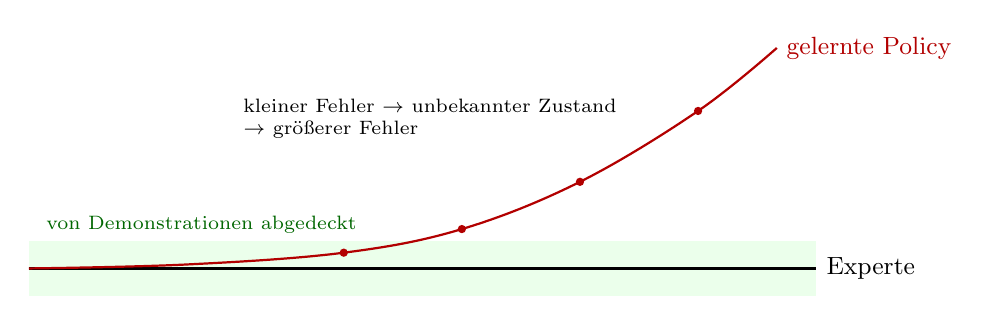
\begin{tikzpicture}[font=\small, x=1cm, y=1cm]
    \fill[green!8] (0,-0.35) rectangle (10,0.35);
    \node[font=\scriptsize, green!40!black, anchor=west] at (0.1,0.55)
      {von Demonstrationen abgedeckt};
    \draw[thick] (0,0) -- (10,0) node[right] {Experte};
    \draw[red!70!black, thick] plot[smooth, tension=0.6] coordinates
      {(0,0) (2,0.05) (4,0.2) (5.5,0.5) (7,1.1) (8.5,2.0) (9.5,2.8)};
    \node[red!70!black, anchor=west] at (9.5,2.8) {gelernte Policy};
    \foreach \x/\y in {4/0.2, 5.5/0.5, 7/1.1, 8.5/2.0} {\fill[red!70!black] (\x,\y) circle (1.5pt);}
    \node[font=\scriptsize, align=left, anchor=west] at (2.6,1.9)
      {kleiner Fehler $\rightarrow$ unbekannter Zustand\\$\rightarrow$ größerer Fehler};
  \end{tikzpicture}
  \caption[Fehlerfortpflanzung beim Behavior Cloning]{Fehlerfortpflanzung beim Behavior
  Cloning (schematisch): Sobald die Policy den von den Demonstrationen abgedeckten Bereich
  verlässt, fehlen ihr Beispiele für die Rückkehr, und die Abweichung wächst.}
  \label{fig:drift}
\end{figure}

Zwei Gegenmaßnahmen sind in der Literatur etabliert:
\begin{description}
  \item[\acs{dagger}] \ac{dagger}~\cite{ross2011} führt die gelernte Policy aus, lässt die
    dabei besuchten Zustände nachträglich vom Experten mit der richtigen Aktion versehen und
    trainiert auf der Vereinigung aller Daten erneut. Das Verfahren erreicht die lineare
    Schranke, braucht aber einen Experten, der in beliebigen Zuständen die richtige Aktion
    angeben kann, und mehrere Runden an der Anlage.
  \item[\acs{dart}] \ac{dart}~\cite{laskey2017} stört bereits die Demonstrationen des
    Experten mit Rauschen. Der Roboter weicht dadurch von der idealen Bahn ab, der Experte
    korrigiert, und die Korrekturen landen als Beispiele im Datensatz. Die Verteilung der
    Trainingsdaten wird so in Richtung der Zustände verbreitert, in die die Policy später
    geraten kann.
\end{description}
Modul~4 setzt \ac{dart} um (\cref{sec:rauschen-mathe}); \ac{dagger} ist als spätere
Erweiterung vorgesehen (\cref{ch:fazit}).

\subsection{Mehrdeutige Lösungen}
\label{sec:multimodal}

Die zweite Hürde betrifft die Wahl der Verlustfunktion. Für den quadratischen Verlust aus
\cref{eq:bc-ziel} ist die optimale Vorhersage der bedingte Erwartungswert
\begin{equation}
  \pi_\theta^{\mathrm{opt}}(o) = \argmin_{\hat a}\; \E\bigl[\lVert \hat a - a\rVert^2 \mid o\bigr]
  = \E[a \mid o] .
  \label{eq:mittelwert}
\end{equation}
Gibt es für dieselbe Beobachtung mehrere richtige Aktionen, etwa links oder rechts an einem
Hindernis vorbei, ist die Verteilung $p(a \mid o)$ \emph{multimodal}, und ihr Mittelwert
liegt zwischen den Moden, unter Umständen mitten im Hindernis. Eine Policy, die die ganze
Verteilung darstellen und daraus ziehen kann, hat dieses Problem nicht. Das ist der Grund für
den Einsatz eines Diffusionsmodells (\cref{sec:diffusion}).

Ein verwandter Fall tritt in Modul~4 an Haltepunkten auf: Steht der Arm still, weil er
gleich losfährt, und steht er still, weil er gerade angekommen ist, ist die Beobachtung
nahezu gleich, die richtige Aktion aber verschieden. Die Policy lernt dann \enquote{stehen
bleiben} (\cref{ch:versuche}).

\subsection{Weitere Hürden}
\label{sec:weitere-huerden}

\begin{description}
  \item[Datenmenge und Datenqualität] Jede Demonstration kostet Zeit an der Anlage. Fehler in
    den Daten, etwa vertauschte Kameras, zeitlich verschobene Bilder oder schwankende
    Belichtung, lernt das Netz ungeprüft mit.
  \item[Konsistenz zwischen Aufnahme und Ausführung] Die Policy kennt nur die Bedingungen der
    Aufnahme. Takt, Bildgröße, Kameraeinstellungen, Geschwindigkeit und Kameraposition müssen
    bei der Ausführung übereinstimmen.
  \item[Echtzeit] Die Vorhersage eines großen Netzes dauert länger als ein Takt. Die
    Ausführung muss damit umgehen, ohne dass der Arm ruckelt oder stehen bleibt.
  \item[Sicherheit] Ein Netz kann beliebige Sollwerte ausgeben. Anders als bei einer
    programmierten Bahn lässt sich das Verhalten nicht vorab vollständig prüfen; jeder Befehl
    muss vor dem Senden geprüft werden.
\end{description}
\Cref{ch:anforderungen} leitet aus diesen Hürden die Anforderungen an Modul~4 ab.

% ==============================================================================
\section{Eingespeistes Rauschen}
\label{sec:rauschen-mathe}

\subsection{Asymmetrische Datenpaare}

Bei \ac{dart} wird die tatsächlich gefahrene Bahn $\tilde x_t = x_t^{*} + \delta_t$ um eine
Störung $\delta_t$ von der idealen Bahn $x_t^{*}$ des Experten ausgelenkt. Gespeichert wird
die Beobachtung des \emph{gestörten} Zustands zusammen mit der Aktion des Experten, die zur
\emph{idealen} Bahn zurückführt:
\begin{equation}
  \bigl(o_t,\, a_t\bigr) = \bigl(o(\tilde x_t),\; x_{t+1}^{*}\bigr) .
  \label{eq:asymm}
\end{equation}
Die Störung selbst kommt in den Aktionen nie vor und wird deshalb nicht mitgelernt. Jedes
Paar enthält dagegen implizit die Korrektur $x_{t+1}^{*} - \tilde x_t$.

\subsection{Ornstein-Uhlenbeck-Prozess}

Würde $\delta_t$ in jedem Takt unabhängig gezogen, sähe die Störung wie ein Zittern aus, das
der Arm wegen seiner Trägheit kaum ausführen kann und das im Bild nicht als Abweichung
erkennbar ist. Modul~4 verwendet deshalb einen Ornstein-Uhlenbeck-Prozess~\cite{uhlenbeck1930},
der als stochastische Differentialgleichung lautet:
\begin{equation}
  \mathrm{d}\delta = -\frac{\delta}{\tau}\,\mathrm{d}t + \sqrt{\frac{2}{\tau}}\;\sigma\,\mathrm{d}W .
  \label{eq:ou-sde}
\end{equation}
Der erste Term zieht die Auslenkung mit der Zeitkonstante $\tau$ zur Null zurück, der zweite
lenkt sie über einen Wiener-Prozess $W$ immer wieder aus. Mit dieser Skalierung hat der
Prozess im eingeschwungenen Zustand die Standardabweichung $\sigma$. Für den Takt $\Delta t$
gilt die exakte Diskretisierung
\begin{equation}
  \delta_{k+1} = \alpha\,\delta_k + \sigma\sqrt{1 - \alpha^2}\;\xi_k,
  \qquad \alpha = e^{-\Delta t / \tau},\quad \xi_k \sim \N(0, I) ,
  \label{eq:ou-diskret}
\end{equation}
und die Autokorrelation fällt exponentiell ab,
$\E[\delta_k \delta_{k+m}] = \sigma^2 \alpha^{|m|}$. Aufeinanderfolgende Auslenkungen sind
also stark korreliert; die Bahn schlingert langsam um die Idealbahn. Modul~4 glättet den
Prozess zusätzlich mit einem kritisch gedämpften Glied zweiter Ordnung, damit auch
Geschwindigkeit und Beschleunigung der Störung begrenzt bleiben
(\cref{sec:noise-umsetzung}).

% ==============================================================================
\section{Diffusionsmodelle}
\label{sec:diffusion}

Diffusionsmodelle~\cite{sohldickstein2015,ho2020} sind generative Modelle: Sie lernen eine
Wahrscheinlichkeitsverteilung $p(x_0)$ aus Beispielen und können daraus neue Proben ziehen.
Das Prinzip besteht aus zwei Prozessen (\cref{fig:diffusion}).

\subsection{Vorwärtsprozess}

Der Vorwärtsprozess zerstört eine Probe $x_0$ in $K$ Schritten durch Gaußsches Rauschen.
Mit einem festen Rauschplan $\beta_1, \dots, \beta_K$ gilt
\begin{equation}
  q(x_k \mid x_{k-1}) = \N\bigl(x_k;\, \sqrt{1-\beta_k}\,x_{k-1},\, \beta_k I\bigr) .
\end{equation}
Mit $\alpha_k = 1 - \beta_k$ und $\bar\alpha_k = \prod_{s=1}^{k}\alpha_s$ lässt sich jeder
Schritt direkt aus $x_0$ angeben:
\begin{equation}
  x_k = \sqrt{\bar\alpha_k}\,x_0 + \sqrt{1-\bar\alpha_k}\;\varepsilon,
  \qquad \varepsilon \sim \N(0, I) .
  \label{eq:forward}
\end{equation}
Für großes $K$ geht $\bar\alpha_K$ gegen null, und $x_K$ ist reines Rauschen.

\subsection{Rückwärtsprozess und Training}

Ein neuronales Netz lernt, den Vorwärtsprozess umzukehren. In der Formulierung von Ho et
al.~\cite{ho2020} sagt es das in $x_k$ enthaltene Rauschen voraus; trainiert wird mit dem
einfachen Verlust
\begin{equation}
  \mathcal{L}_\varepsilon = \E_{x_0,\,k,\,\varepsilon}
    \Bigl[\bigl\lVert \varepsilon - \varepsilon_\theta(x_k, k) \bigr\rVert^2\Bigr] .
  \label{eq:loss-eps}
\end{equation}
Gleichwertig kann das Netz die unverrauschte Probe direkt vorhersagen,
\begin{equation}
  \mathcal{L}_{x_0} = \E_{x_0,\,k,\,\varepsilon}
    \Bigl[\bigl\lVert x_0 - \hat x_\theta(x_k, k) \bigr\rVert^2\Bigr],
  \label{eq:loss-x0}
\end{equation}
denn über \cref{eq:forward} lassen sich $\varepsilon$ und $x_0$ ineinander umrechnen. Welche
Variante besser funktioniert, hängt von der Anwendung ab; Modul~4 verwendet aus den in
\cref{ch:training} beschriebenen Gründen \cref{eq:loss-x0}.

Zur Erzeugung beginnt man bei $x_K \sim \N(0, I)$ und wendet das Netz schrittweise an. Ein
Schritt des \ac{ddpm} lautet
\begin{equation}
  x_{k-1} = \frac{1}{\sqrt{\alpha_k}}
    \Bigl( x_k - \frac{\beta_k}{\sqrt{1-\bar\alpha_k}}\,\varepsilon_\theta(x_k, k) \Bigr)
    + \sigma_k z, \qquad z \sim \N(0, I) .
  \label{eq:ddpm-step}
\end{equation}
Anschaulich verschiebt jeder Schritt die Probe ein Stück in Richtung höherer
Wahrscheinlichkeit der gelernten Verteilung. Weil die Erzeugung bei Zufall beginnt, landen
verschiedene Durchläufe in verschiedenen Moden der Verteilung, statt zwischen ihnen zu mitteln
(\cref{sec:multimodal}).

\begin{figure}[htbp]
  \centering
  \begin{tikzpicture}[font=\small, x=1cm, y=1cm]
    \foreach \i/\n/\lbl in {0/0/$x_0$, 1/0.35/$x_1$, 2/0.7/$\cdots$, 3/1/$x_K$} {
      \begin{scope}[shift={(\i*3.6,0)}]
        \draw[black!30] (0,-1) rectangle (2.4,1);
        \draw[thick, blue!70!black] plot[smooth, tension=0.6] coordinates
          {(0.2,-0.6) (0.8,{-0.2+\n*0.5}) (1.4,{0.3-\n*0.8}) (2.2,{0.7-\n*1.1})};
        \foreach \p in {1,...,14} {
          \pgfmathsetmacro{\px}{0.15+rnd*2.1}
          \pgfmathsetmacro{\py}{-0.9+rnd*1.8}
          \fill[black!50, opacity=\n] (\px,\py) circle (0.8pt);
        }
        \node at (1.2,-1.3) {\lbl};
      \end{scope}
    }
    \draw[-{Stealth[length=2mm]}, thick] (0.6,1.3) -- node[above] {Vorwärtsprozess $q$: Rauschen hinzufügen} (11.4,1.3);
    \draw[-{Stealth[length=2mm]}, thick, blue!70!black] (11.4,-1.9) -- node[below] {Rückwärtsprozess $p_\theta$: schrittweise entrauschen (gelernt)} (0.6,-1.9);
  \end{tikzpicture}
  \caption[Vorwärts- und Rückwärtsprozess eines Diffusionsmodells]{Vorwärts- und
  Rückwärtsprozess eines Diffusionsmodells am Beispiel einer Aktionsfolge (blaue Kurve).
  Der Vorwärtsprozess überdeckt sie schrittweise mit Rauschen, der gelernte Rückwärtsprozess
  stellt aus reinem Rauschen eine plausible Folge her.}
  \label{fig:diffusion}
\end{figure}

\subsection{Beschleunigte Erzeugung}

Mit $K = 100$ Schritten ist die Erzeugung für eine Robotersteuerung zu langsam.
\ac{ddim}~\cite{song2021} verwendet dasselbe trainierte Netz, ersetzt den stochastischen
Schritt aber durch einen deterministischen, der Zwischenschritte überspringen kann. Mit der
Schätzung $\hat x_0$ aus dem aktuellen Schritt lautet der Sprung von $k$ nach $k' < k$
\begin{equation}
  x_{k'} = \sqrt{\bar\alpha_{k'}}\;\hat x_0
         + \sqrt{1-\bar\alpha_{k'}}\;\hat\varepsilon,
  \qquad \hat\varepsilon = \frac{x_k - \sqrt{\bar\alpha_k}\,\hat x_0}{\sqrt{1-\bar\alpha_k}} .
  \label{eq:ddim}
\end{equation}
Modul~4 trainiert mit 100 Schritten und erzeugt mit 10 \ac{ddim}-Schritten, was die
Rechenzeit etwa um den Faktor zehn verkürzt.

% ==============================================================================
\section{Diffusion Policy}
\label{sec:dp}

\subsection{Bedingte Erzeugung von Aktionsfolgen}

Die \ac{dp}~\cite{chi2024} überträgt das Diffusionsprinzip auf die Robotersteuerung. Die
erzeugte Probe ist eine Folge von $T_p$ zukünftigen Aktionen
$A_t = (a_t, \dots, a_{t+T_p-1})$, und das Netz erhält zusätzlich die letzten $T_o$
Beobachtungen $O_t = (o_{t-T_o+1}, \dots, o_t)$ als Bedingung. Gelernt wird damit die bedingte
Verteilung $p(A_t \mid O_t)$, der Verlust aus \cref{eq:loss-x0} wird zu
\begin{equation}
  \mathcal{L} = \E_{(O_t, A_t) \sim \mathcal{D},\,k,\,\varepsilon}
    \Bigl[\bigl\lVert A_t - \hat A_\theta\bigl(\sqrt{\bar\alpha_k}A_t
      + \sqrt{1-\bar\alpha_k}\,\varepsilon,\; k,\; O_t\bigr)\bigr\rVert^2\Bigr] .
  \label{eq:loss-dp}
\end{equation}

\Cref{fig:dp-netz} zeigt den Aufbau. Jedes Kamerabild wird von einem eigenen \ac{cnn}, in
Modul~4 einem ResNet18~\cite{he2016}, in einen Merkmalsvektor übersetzt. Die Merkmale aller
Kameras und Takte werden mit dem Roboterzustand zu einem Bedingungsvektor verbunden. Das
eigentliche Entrauschungsnetz ist ein eindimensionales U-Net~\cite{ronneberger2015}, das
entlang der Zeitachse der Aktionsfolge faltet. Der Bedingungsvektor und der Diffusionsschritt
$k$ gehen über FiLM-Schichten~\cite{perez2018} in jeden Block ein: Sie skalieren und
verschieben die Merkmalskanäle,
\begin{equation}
  \mathrm{FiLM}(h) = \gamma(c) \odot h + \beta(c) ,
\end{equation}
wobei $\gamma$ und $\beta$ aus dem Bedingungsvektor $c$ gelernt werden.

\begin{figure}[htbp]
  \centering
  \begin{tikzpicture}[font=\small, node distance=5mm and 6mm,
      blk/.style={draw, rounded corners=1.5mm, align=center, minimum height=9mm, fill=white},
      arr/.style={-{Stealth[length=2mm]}, thick}]
    \node[blk, fill=black!6, text width=24mm] (iw) {Handgelenk\-kamera\\$240\times320$};
    \node[blk, fill=black!6, text width=24mm, below=of iw] (is) {Szenen\-kamera\\$240\times320$};
    \node[blk, fill=black!6, text width=24mm, below=of is] (st) {Zustand (14)};
    \node[blk, right=of iw, text width=20mm] (rw) {ResNet18};
    \node[blk, right=of is, text width=20mm] (rs) {ResNet18};
    \node[blk, fill=orange!12, right=of rs, text width=22mm, minimum height=40mm] (c)
      {Bedingung $c$\\(2 Takte)};
    \draw[arr] (iw) -- (rw); \draw[arr] (is) -- (rs);
    \draw[arr] (rw) -- (rw -| c.west); \draw[arr] (rs) -- (c);
    \draw[arr] (st) -- (st -| c.west);
    \node[blk, fill=blue!8, right=10mm of c, text width=30mm, minimum height=40mm] (unet)
      {1D-U-Net\\[2mm] $\hat A_\theta(A^{(k)}, k, c)$};
    \draw[arr] (c) -- node[above, font=\scriptsize] {FiLM} (unet);
    \node[blk, above=8mm of unet, text width=30mm] (noise) {$A^{(k)}$, verrauschte Folge};
    \draw[arr] (noise) -- (unet);
    \node[blk, fill=green!10, below=8mm of unet, text width=30mm] (out) {Aktionsfolge\\$16 \times 7$};
    \draw[arr] (unet) -- (out);
    \draw[arr, densely dashed] (unet.east) -- ++(5mm,0) |- node[pos=0.25, right, font=\scriptsize,
      align=left] {10 Schritte\\(\acs{ddim})} (noise.east);
  \end{tikzpicture}
  \caption[Aufbau der Diffusion Policy]{Aufbau der Diffusion Policy in Modul~4. Die Bilder
  beider Kameras und der Zustand der letzten zwei Takte bilden die Bedingung; das U-Net
  entrauscht daraus in zehn Schritten eine Folge von 16 Aktionen.}
  \label{fig:dp-netz}
\end{figure}

\subsection{Ausführung mit überlappenden Aktionsfolgen}

Von den $T_p$ vorhergesagten Aktionen werden nur die ersten $T_a < T_p$ ausgeführt, dann
wird mit einer neuen Beobachtung erneut vorhergesagt (Receding Horizon). Die Folge sorgt für
eine gleichmäßige Bewegung über mehrere Takte, die häufige Neuvorhersage für die Reaktion auf
Änderungen. Wird öfter neu vorhergesagt, als Aktionen ausgeführt werden, liegen für denselben
Takt mehrere Vorhersagen vor. Zhao et al.~\cite{zhao2023} mitteln sie (Temporal Ensembling):
\begin{equation}
  a_t = \frac{\sum_{j} w_j\, \hat a_t^{(j)}}{\sum_j w_j},
  \qquad w_j = e^{-m\,j},
  \label{eq:ensemble}
\end{equation}
wobei $\hat a_t^{(j)}$ die Vorhersage für Takt $t$ aus der $j$-ältesten Folge ist. Modul~4
verwendet $m = 0$, also einen ungewichteten Mittelwert. Die konkrete Taktung beschreibt
\cref{ch:ausfuehrung}.

\subsection{Bibliothek LeRobot}

Modul~4 verwendet die Umsetzung der Diffusion Policy aus der Bibliothek
LeRobot~\cite{lerobot} in Version~0.6.1. LeRobot legt außerdem ein Datensatzformat fest, in
dem Zustände, Aktionen und Kamerabilder einer Demonstration mit gemeinsamen Zeitstempeln
gespeichert werden (\cref{ch:datenaufnahme}).
